% Realizada por César Martínez cesar.martinez@udlap.mx
%VERSION 2.0


\documentclass[12pt]{article}  %tipo de documento y tamaño de letra normal
%%%%%%%%%%%%%%%%%%%%%%%%%%%%%%%%%%%%%%%%%%%%%%%%%%%%%%%%%%%%%%%%%%%%%
%%%%%%%%%%%%%%%%%%%%%%%%%%%%%%%%%%%%%%%%%%%%%%%%%%%%%%%%%%%%%%%%%%%%%
%%%%%%%%%%%%%%%%%%%%%%%%%%%%%%%%%%%%%%%%%%%%%%%%%%%%%%%%%%%%%%%%%%%%%
%%%%%%%% Paquetes basicos, pueden encontrar información especifica de cada uno de ellos en  (https://www.ctan.org/) %%%%%%%%%%%%%%%%%%%%%%% %%%%%%%%%%%%%%%%%%%%%%%%%%%%%%%%%%%%%%%%%%%%%%%%%%%%%%%%%%%%%%%%%%%%%
%%%%%%%%%%%%%%%%%%%%%%%%%%%%%%%%%%%%%%%%%%%%%%%%%%%%%%%%%%%%%%%%%%%%%
%%%%%%%%%%%%%%%%%%%%%%%%%%%%%%%%%%%%%%%%%%%%%%%%%%%%%%%%%%%%%%%%%%%%%
\usepackage[spanish]{babel} %Indica que escribiermos en español
%\usepackage[english]{babel} %Indica que escribiermos en inglés
%Comentar la línea del idiona que NO usarán en su reporte
\usepackage[utf8]{inputenc} %Indica qué codificación se está usando ISO-8859-1(latin1)  o utf8  
\usepackage{amsmath} % Comandos extras para matemáticas (cajas para ecuaciones,etc)
\usepackage{amssymb} % Simbolos matematicos (por lo tanto)
\usepackage{graphicx} % Incluir imágenes en LaTeX
\usepackage{color} % Para colorear texto
\usepackage{subfigure} % subfiguras
\usepackage{enumerate} % enumerar
\usepackage{commath} % funcionalidades extras para diferenciales, integrales,etc (\od, \dif, etc)
\usepackage{cancel} % para cancelar expresiones (\cancelto{0}{x})
\usepackage{float} %Podemos usar el especificador [H] en las figuras para que se queden donde queramos
\usepackage{appendix} %Para crear apendices
\usepackage{xcolor} %Definir colores personalizados
%%%%%%%%%%%%%%%%%%%%%%%%%%%%%%%%%%%%%%%%%%%%%%%%%%%%%%%%%%%%%%%%%%%%%
%%%%%%%%% PAQUETES CON OPCIONES ESPECIFICAS PRECARGADAS %%%%%%%%%%%%%
%%%%%%%%%%%%%%%%%%%%%%%%%%%%%%%%%%%%%%%%%%%%%%%%%%%%%%%%%%%%%%%%%%%%%
%%%%%%%%%%%%% Permitir agregar código, colocarlo en un rectángulo y  numerarlo %%%%%%%%%%%%%%%%%%%%%%%%%%%%%%%%%%%%%%%%%%%%%%%%%%%%%%%%%%%
%%%%%%%%%%%%%%%%%%%%%%%%%%%%%%%%%%%%%%%%%%%%%%%%%%%%%%%%%%%%%%%%%%%%%
%%%%%%%%%%%%%%%%%%%%%%%%%%%%%%%%%%%%%%%%%%%%%%%%%%%%%%%%%%%%%%%%%%%%%%%%%%%%%%%%%%%%%%%%%%%%%%%%%%%%%%%%%%%%%%%%%%%%%%%%%%%%%%%%%%%%%%%%%%
\usepackage{listings} %Sirve para pegar codigo fuente de programas
\usepackage{caption} %Agregar titulos a los codigos
\DeclareCaptionFont{white}{\color{white}}
\DeclareCaptionFormat{listing}{%
  \parbox{\textwidth}{\colorbox{gray}{\parbox{\textwidth}{#1#2#3}}\vskip-4pt}}
\captionsetup[lstlisting]{format=listing,labelfont=white,textfont=white}
\lstset{frame=lrb,xleftmargin=\fboxsep,xrightmargin=-\fboxsep}
\renewcommand{\lstlistingname}{Código}
%%%%%%%%%%%%%%%%%%%%%%%%%%%%%%%%%%%%%%%%%%%%%%%%%%%%%%%%%%%%%%%%%%%%%
%%% Definir márgenes del documento%%%%%%%%%%%%%%%%%%%%%%%%%%%%%%%%%%%
%%%%%%%%%%%%%%%%%%%%%%%%%%%%%%%%%%%%%%%%%%%%%%%%%%%%%%%%%%%%%%%%%%%%%
 \usepackage{anysize} % Para personalizar el ancho de  los márgenes
\marginsize{2cm}{2cm}{2cm}{2cm} % Izquierda, derecha, arriba, abajo
%%%%%%%%%%%%%%%%%%%%%%%%%%%%%%%%%%%%%%%%%%%%%%%%%%%%%%%%%%%%%%%%%%%%
%%% Hipervinculos activos y a color %%%%%%%%%%%%%%%%%%%%%%%%%%%%%%%%
%%%%%%%%%%%%%%%%%%%%%%%%%%%%%%%%%%%%%%%%%%%%%%%%%%%%%%%%%%%%%%%%%%%%%
\usepackage[colorlinks=true,plainpages=true,citecolor=blue,linkcolor=black]{hyperref}
\usepackage{hyperref} 
%%%%%%%%%%%%%%%%%%%%%%%%%%%%%%%%%%%%%%%%%%%%%%%%%%%%%%%%%%%%%%%%%%%%%
%%%%%% Encabezado y pie de pagina %%%%%%%%%%%%%%%%%%%%%%%%%%%%%%%%%%%
%%%%%%%%%%%%%%%%%%%%%%%%%%%%%%%%%%%%%%%%%%%%%%%%%%%%%%%%%%%%%%%%%%%%%
\usepackage{fancyhdr} 
\pagestyle{fancy}
\fancyhf{}
\fancyhead[L]{\footnotesize UDLAP} %encabezado izquierda
\fancyhead[R]{\footnotesize CEM}   % encabezado derecha
\fancyfoot[R]{\footnotesize \curso}  % Pie derecha
\fancyfoot[C]{\thepage}  % centro
\fancyfoot[L]{}  %izquierda
\renewcommand{\footrulewidth}{0.4pt}
%%%%%%%%%%%%%%%%%%%%%%%%%%%%%%%%%%%%%%%%%%%%%%%%%%%%%%%%%%%%%%%%%%%%%
%%%% Carpeta donde se deben colocar las imagenes %%%%%%%%%%%%%%%%%%%%
\graphicspath{{Imagenes/}} %Colocar aqui todas las imagenes del documento pueden estar en formato png, eps o jpg, se recomienda eps para mayor calidad.
%%%%%%%%%%%%%%%%%%%%%%%%%%%%%%%%%%%%%%%%%%%%%%%%%%%%%%%%%%%%%%%%%%%%%
%%%%%%%%%%%%%%%%%%%%%%%%%%%%%%%%%%%%%%%%%%%%%%%%%%%%%%%%%%%%%%%%%%%%%
%%%%%%%% Termina carga de paquetes %%%%%%%%%%%%%%%%%%%%%%%%%%%%%%%%%%
%%%%%%%%%%%%%%%%%%%%%%%%%%%%%%%%%%%%%%%%%%%%%%%%%%%%%%%%%%%%%%%%%%%%%
%%%%%%%%%%%%%%%%%%%%%%%%%%%%%%%%%%%%%%%%%%%%%%%%%%%%%%%%%%%%%%%%%%%%%
%%%%%%%%%%%%%%%%%%%%%%%%%%%%%%%%%%%%%%%%%%%%%%%%%%%%%%%%%%%%%%%%%%%%%
%%%%%% Modificar campos que aparecerán en portada %%%%%%%%%%%%%%%%%%%
%%%%%%%%%%%%%%%%%%%%%%%%%%%%%%%%%%%%%%%%%%%%%%%%%%%%%%%%%%%%%%%%%%%%%
%%%%%%%%%%%%%%%%%%%%%%%%%%%%%%%%%%%%%%%%%%%%%%%%%%%%%%%%%%%%%%%%%%%%%
%%%%%%%%%%%%%%%%%%%%%%%%%%%%%%%%%%%%%%%%%%%%%%%%%%%%%%%%%%%%%%%%%%%%%
\def\titulo{Reporte final: Máquina expendedora de golosinas}%titulo del documento
\def\materia{Clave materia sección: LRT2022-1} %Clave nombre de la materia y sección
\def\curso{Diseño Digital} %Nombre de la materia para footnote
\def\fecha{27 de Noviembre de 2023} %En formato "dia" de "mes" de "año"
\def\equipo {1}%Verificar en blackboard el número asignado
\def\ida{177516} %Nombre y Id´s de todos los integrantes que hayan trabajado en el proyecto
\def\esta{Jesus Alvarez Sombrerero}
\def\idb{177485}
\def\estb{Iván Estrella Sánchez}
\def\idc{178432}
\def\estc{Fernanda Sofía Ovalle Prado}
\def\idd{177212}
\def\estd{Daniel Yamil Tlilayatzi Muñoz}
%%%%%%%%%%%%%%%%%%%%%%%%%%%%%%%%%%%%%%%%%%%%%%%%%%%%%%%%%%%%%%%%%%%%%
%%%%%%%%%%%%%%%%%%%%%%%%%%%%%%%%%%%%%%%%%%%%%%%%%%%%%%%%%%%%%%%%%%%%%
%%%%%%%%%%%%%%%%%%%%%%%%%%%%%%%%%%%%%%%%%%%%%%%%%%%%%%%%%%%%%%%%%%%%%
\begin{document} %Inicia el documento
%%%%%%%%%%%%%%%%%%%%%%%%%%%%%%%%%%%%%%%%%%%%%%%%%%%%%%%%%%%%%%%%%%%%%
%%%%%%%%%%%%%%%%%%%%%%%%%%%%%%%%%%%%%%%%%%%%%%%%%%%%%%%%%%%%%%%%%%%%%
%%%%%%%%%%%%%%%%%%%%%%%%%%%%%%%%%%%%%%%%%%%%%%%%%%%%%%%%%%%%%%%%%%%%%
%%%%%%%%%%%%%%%%%%%%%%%%%%%%%%%%%% PORTADA %%%%%%%%%%%%%%%%%%%%%%%%%%
%%%%%%%%%%%%%%%%%%%%%%%%%%%%%%%%%%%%%%%%%%%%%%%%%%%%%%%%%%%%%%%%%%%%%No es necesario modificar ninguna de las siguientes lineas, sólo si el número de estudiantes que conforman su equipo es menor o mayor a 5
%%%%%%%%%%%%%%%%%%%%%%%%%%%%%%%%%%%%%%%%%%%%%%%%%%%%%%%%%%%%%%%%%%%%%
%%%%%%%%%%%%%%%%%%%%%%%%%%%%%%%%%%%%%%%%%%%%%%%%%%%%%%%%%%%%%%%%%%%%%
%%%%%%%%%%%%%%%%%%%%%%%%%%%%%%%%%%%%%%%%%%%%%%%%%%%%%%%%%%%%%%%%%%%%%
\begin{center}
  \newcommand{\HRule}{\rule{\linewidth}{0.5mm}}
  \thispagestyle{empty}
  \vspace*{-1.5cm}
  \textsc{\huge Universidad de las Américas Puebla}\\[1.5cm]
  \textsc{\LARGE Escuela de ingeniería}\\[1.5cm]
  \textsc{\LARGE Departamento de computación, electrónica y mecatrónica}\\[1.5cm]
  \includegraphics[width=150mm]{UDLAP}  									\vspace*{1cm}														\HRule \\[0.4cm]
  { \huge \bfseries \titulo}\\[0.4cm]
  \HRule \\[1cm]
  { \Large \bfseries \materia}\\[1cm]
  { \Large \bfseries Equipo \equipo}\\[1cm]
  \begin{flushleft} \Large
    \ida \hspace{0.5cm}\esta \\
    \idb \hspace{0.5cm}\estb \\
    \idc \hspace{0.5cm}\estc \\
    \idd \hspace{0.5cm}\estd \\ %Copiar y pegar más líneas si su equipo tiene más de 5 integrantes, eliminar si está formado por menos
  \end{flushleft}
  \vfill
  \begin{center}
    {\Large A \fecha, San Andrés Cholula, Puebla}
  \end{center}
\end{center}							 								\newpage
%%%%%%%%%%%%%%%%%%%% TERMINA PORTADA %%%%%%%%%%%%%%%%%%%%%%%%%%%%%%%%
%%%%%%%%%%%%%%%%%%%%%%%%%%%%%%%%%%%%%%%%%%%%%%%%%%%%%%%%%%%%%%%%%%%%%
%%%%%%%%%%%%%%%%%%%%%%%%%%%%%%%%%%%%%%%%%%%%%%%%%%%%%%%%%%%%%%%%%%%%%
%%%%%%%%%%%%%%%%%%%%%%%%%%%%%%%%%%%%%%%%%%%%%%%%%%%%%%%%%%%%%%%%%%%%%
%%%%%%%%%%%%%%%%%%%%%%%%%%%%%%%%%%%%%%%%%%%%%%%%%%%%%%%%%%%%%%%%%%%%%
\thispagestyle{empty} %Para no numerar la página del indice
\tableofcontents %Comando que genera el índice
\newpage %Se asegura que el documento inicie en la sigueinte pagina despues del índice
\setcounter{page}{1} %Para comenzaMaquina expendedora de golosinasr a numerar las páginas desde este punto
\section{Objetivo y objetivos particulares}
Programar y simular un circuito secuencial que controle una máquina expendedora.
\subsection{Objetivos particulares}
\begin{itemize}
  \item La máquina debe permitir comprar 5 productos.
  \item La máquina admite monedas de 1, 2, 5 y 10 pesos únicas.
  \item La máquina permite confirmar la compra, además de solicitar el cambio.
  \item La máquina debe tener un botón de reset que igual sirve para cancelar.
  \item Diseñar un circuito que permita la simulación de la máquina.
  \item Programar el circuito en un FPGA Basys 3 utilizando VHDL.
  \item Realizar testbench para verificar el funcionamiento del circuito en EDA Playground.
\end{itemize}

\section*{Materiales}

\subsection*{Equipamiento}

\begin{itemize}
  \item Basys 3 board
\end{itemize}

\subsection*{Software}

\begin{itemize}
  \item Vivado 2022.2
  \item EDA Playground
\end{itemize}

\section{Introducción y Marco Teórico}
El proyecto aborda el diseño y la simulación de un circuito secuencial para controlar una máquina expendedora, utilizando el lenguaje de programación VHDL y el hardware FPGA Basys 3. El objetivo principal es crear un sistema que administre la venta de cinco productos diferentes: picafresa, 3 pesos; ositos, 6 pesos; viboritas, 7 pesos; papas, 12 pesos; jugo, 15 pesos.Este acepta monedas de 1, 2, 5 y 10 pesos que no se repiten. El diseño debe incluir funcionalidades clave, como la confirmación de compra, solicitud de cambio, y un botón de reset que también sirve para cancelar transacciones. Se busca probar todo con un testbench en EDA Playground y luego pasarlo a Vivado para programarlo en el Basys 3. Por cuestiones de tamaño de archivo, se omitirá el apéndice y se pasará a colocar los códigos e imágenes en el reporte directamente.

Un circuito secuencial es un tipo de circuito eléctrico en el que la salida no solo depende de las entradas actuales, sino también del historial de entradas anteriores. A diferencia de los circuitos combinacionales, donde la salida es una función directa de las entradas, los circuitos secuenciales incorporan memoria. Esta memoria se logra mediante el uso de elementos de almacenamiento, como flip-flops o latches, que pueden mantener un estado. Esto permite que el circuito "recuerde" información pasada, lo que es fundamental para la creación de dispositivos como computadoras, donde se necesitan secuencias de operaciones y almacenamiento de datos \cite{7169287}.

Una forma que otros han desarrollado una máquina expendedora en VHDL es mediante la implementación de un controlador que gestiona las entradas monetarias y coordina la dispensación de productos y el cambio. Este enfoque utiliza un conjunto de señales para detectar la inserción de dinero y activa la entrega del artículo una vez que se alcanza la cantidad exacta. Con un diseño que incorpora estados de espera y procesamiento, el sistema asegura una operación fluida y eficiente, ajustando las salidas de la máquina en respuesta a las acciones del usuario. La programación en VHDL permite una descripción precisa del comportamiento del controlador de la máquina expendedora \cite{lameres2019quick}.

Siguiendo el acercamiento de seleccionar de acuerdo a casos, decidimos ir por una programación de asignación de señales condicional, además de utilizar la operación de suma y resta con números, contando igual, con un circuito capaz de hacer display de 7 segmentos. En VHDL, la programación de circuitos que realizan operaciones basadas en señales condicionales a menudo sigue un patrón donde un proceso secuencial verifica el estado de múltiples señales de entrada y realiza cálculos o toma decisiones basadas en esos estados. Cada señal de entrada representa una condición o un valor que, cuando es activado, desencadena una acción dentro del proceso. Por su lado las bibliotecas IEEE.STD\_LOGIC\_ARITH y IEEE.STD\_LOGIC\_UNSIGNED son paquetes adicionales en VHDL que proporcionan funcionalidades para realizar operaciones aritméticas con señales que son de tipo std\_logic\_vector \cite{unlp2018}. Por su lado, un display de 7 segmentos en una Basys 3 debe ser mapeado por código utilizando el reloj, se debe diseñar las asignaciones que se pueden realizar en un display y un controlador que recorra los 4 displays. Posteriormente, se debe definir ese controlador en un archivo .xdc junto a los puertos que se pueden utilizar, los cuales deben ser activados en los tipos de asignaciones que se definen \cite{digilent2023}.

\section{Procedimiento}
Este proyecto tuvo dificultades e inicialmente se buscó utilizar un acercamiento de compuertas lógicas. Sin embargo, se entendieron las dificultades de este método y por eso se optó por un método secuencial y de asignación de señales condicional para la solución de este.

\subsection{Diagramas}
Los diagramas buscan ese acercamiento secuencial. Por eso son diagramas que describen los pasos que seguirá el software. Además toman en cuenta el método de utilizar números enteros en vez de standard logic para las operaciones ya que no se utilizan esos bits en compuertas para hacer sumas y restas, simplemente se guían esos datos de bits.

\newpage

\subsubsection{Selector de productos}
El selector de productos busca como objetivo solo activar. Es por eso que las intersecciones representan el caso en el que permiten pasar la señal del valor. Cuando los productos de menor valor son seleccionados, son mandados como prioridad. Sin embargo, la única forma de que otras señales se manden es que los estados de arriba estén desactivados.

\begin{figure}[!ht]
  \centering
  \caption{Diagrama del selector de productos}
  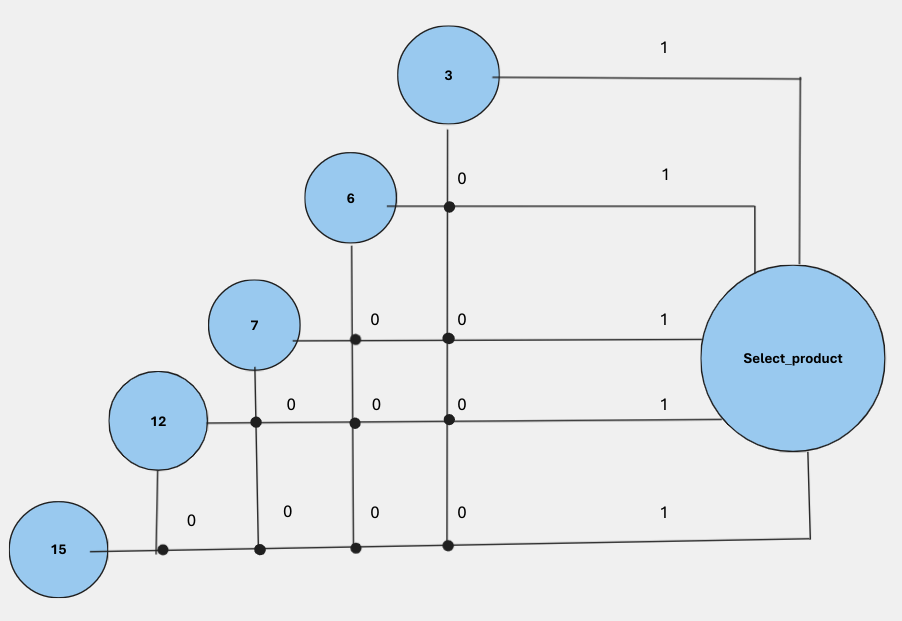
\includegraphics[width=0.25\linewidth]{Imagenes/Diagramas/product-selector-diagram.png}
\end{figure}

\subsubsection{Selector de monedas}
El selector de monedas se puede considerar como botones, la lógica de moneda única la maneja el port al Basys 3 físico. Este circuito tiene como principal punto que cuando su estado es activo(1) se activa su valor y se manda a coin\_total.

\begin{figure}[!ht]
  \centering
  \caption{Diagrama del selector de monedas}
  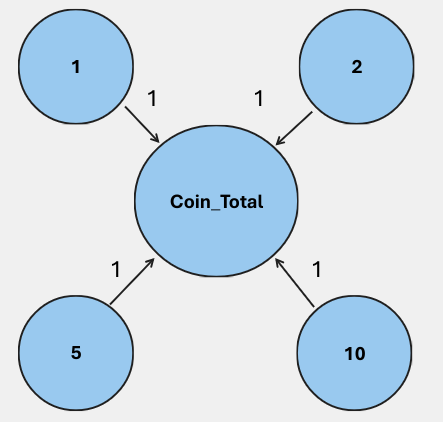
\includegraphics[width=0.25\linewidth]{Imagenes/Diagramas/coin-selector-diagram.png}
\end{figure}

\subsubsection{Calculadora de cambio}
La calculadora de cambio se encarga de recibir 2 int ya convertidos por parte de los dos definidos previamente y realiza operaciones de resta con ellos.

\begin{figure}[!ht]
  \centering
  \caption{Diagrama de la calculadora de cambio}
  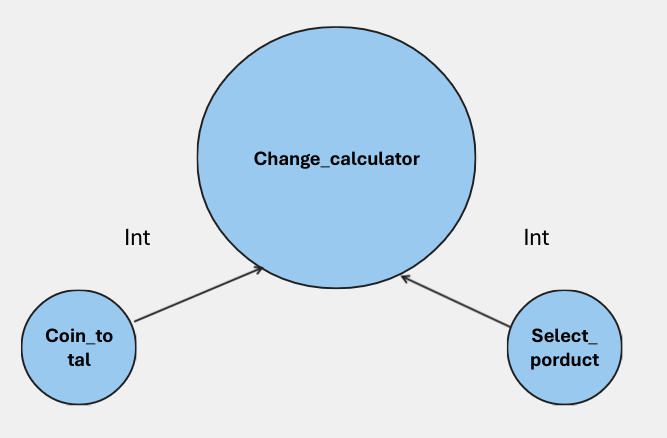
\includegraphics[width=0.25\linewidth]{Imagenes/Diagramas/change-calculator-diagram.png}
\end{figure}

\newpage

\subsubsection{Flip Flop T modificado}
El flip flop T es un circuito secuencial más apegado a lo tradicional. Busca interpretar el procedimiento que lleva el flip flop, dejando de lado la señal de reloj ya que esta es tan rápida en el circuito físico que se puede considerar como un estado constante. Por eso, se utiliza un estado de reset para que el circuito se reinicie y se pueda volver a utilizar. Básicamente, T solo puede ser 0 cuando R se activa. Q se activa con T. Si R es 0, Q manda a R un 1 cuando se activa, lo cual R decide si mantener Q encendida mandando un 1 o apagarla mandando el 0 a T.

\begin{figure}[!ht]
  \centering
  \caption{Diagrama del flip flop T modificado}
  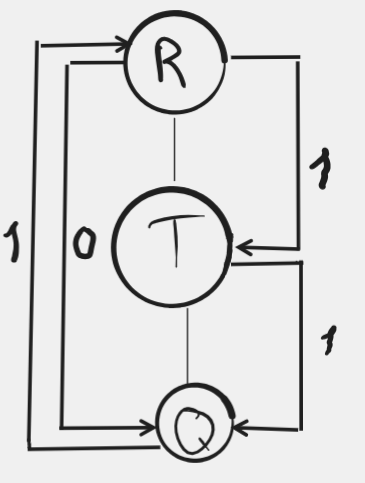
\includegraphics[width=0.25\linewidth]{Imagenes/Diagramas/Flipflop.png}
\end{figure}

\subsubsection{Display de 7 segmentos}
El diagrama del display de 7 segmentos es tomado del libro de referencia del Basys 3. Este explica que se debe hacer un mapeo de los displays utilizando un solo vector que represente lo que se debe mostrar. El controlador de mapeo se debe encargar de utilizar ese vector y modificarlo dependiendo el display.

\begin{figure}[!ht]
  \centering
  \caption{Diagrama del display de 7 segmentos \cite{digilent2023}}
  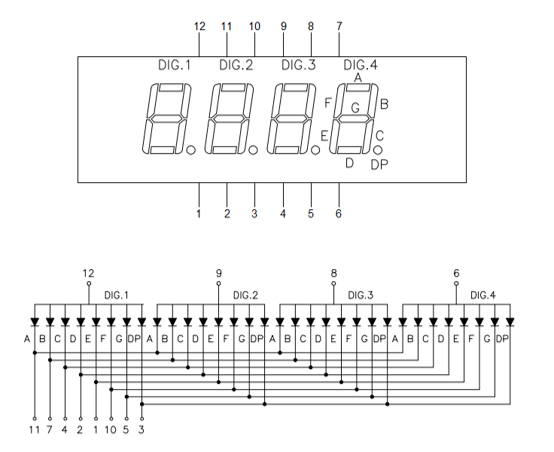
\includegraphics[width=0.25\linewidth]{Imagenes/Diagramas/7seg.png}
\end{figure}

\newpage

\subsubsection{Máquina expendedora}
La máquina busca conectar que el reset reinicie compras. Que solo cuando se confirma la compra y conseguir cambio se pueda mostrar el cambio con el producto comprado y que de no ser el caso se muestre el producto y las monedas totales que se han seleccionado. Este diagrama ilustra de forma el componente general utilizando los componentes antes definidos.

\begin{figure}[!ht]
  \centering
  \caption{Diagrama de la máquina expendedora}
  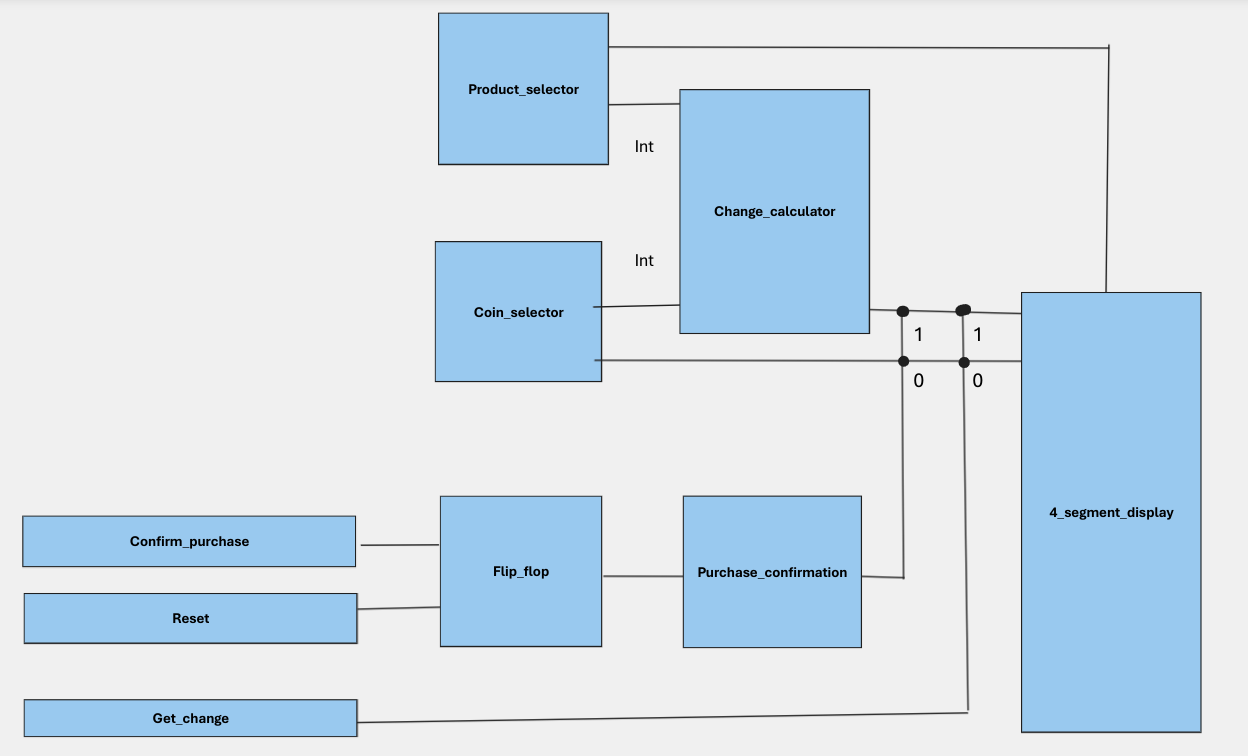
\includegraphics[width=0.25\linewidth]{Imagenes/Diagramas/vending-machine-diagram.png}
\end{figure}

\subsection{Códigos}
La siguiente parte que seguimos fue desarrollar cada componente en VHDL. Para esto, se utilizó el software EDA Playground para simular el funcionamiento de cada componente. Buscamos probar cada componente y ver que funcionara. Decidimos que el componente final era poco apto para simular debido a la cantidad de inputs así que decidimos dejar la prueba a solo el Basys 3. El método de programación que vimos más apto fue el de asignación de señales condicional. Esto debido a que el método de compuertas lógicas era muy complicado de implementar y no era tan eficiente como el de asignación de señales condicional. Además, el método de compuertas lógicas no permitía la utilización de números enteros, lo cual era necesario para la suma y resta de los valores de los productos y el cambio. Básicamente se evitó utilizar un full-adder que hubiera complicado el desarrollo.

\subsubsection{Selector de productos}
El selector de productos es un componente que se encarga de recibir 5 señales de entrada y mandar una señal de salida. Esta señal de salida es la que se encarga de activar el producto que se seleccionó. El selector de productos se encarga de activar el producto de menor valor primero. Esto se logra con la utilización de un if-else. El if-else se encarga de verificar si el producto de menor valor está activo. Si lo está, se activa la señal de salida. Si no, se verifica el siguiente producto de mayor valor. Esto se repite hasta que se activa la señal de salida. El código del selector de productos es el siguiente:

\lstinputlisting[language=VHDL,caption=Selector de productos]{codigos/vhdl/product_selector.vhd}

Procedimos a probar con los testbench los 5 productos y seleccionar dos al mismo tiempo para ver que sí funcionaba la lógica de selección.

\lstinputlisting[language=VHDL,caption=Selector de productos testbench]{codigos/testbench/product_selector_test.vhd}

Con las EPWaves pudimos comprobar que los casos de prueba funcionaban correctamente.

\begin{figure}[!ht]
  \centering
  \caption{EPWaves del selector de productos}
  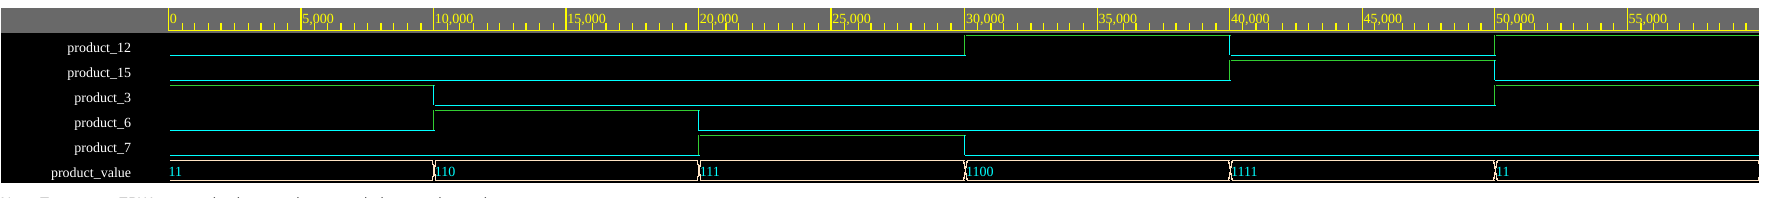
\includegraphics[width=0.75\linewidth]{Imagenes/EPWaves/product-selector-wave.png}
\end{figure}

\newpage

\subsubsection{Selector de monedas}
El selector de monedas es un componente que se encarga de recibir 4 señales de entrada y mandar una señal de salida. Esta señal de salida es la que se encarga de activar la moneda que se seleccionó. El selector de monedas se encarga de activar la moneda de menor valor primero. Este se hizo utilizando solo if sin else para lograr seleccionar todos y de manera única. El código del selector de monedas es el siguiente:

\lstinputlisting[language=VHDL,caption=Selector de monedas]{codigos/vhdl/coin_selector.vhd}

Procedimos a probar con los testbench las monedas solas y otros casos seleccionar más de una. Sin embargo, por temas desconocidos de UTF-8 de LaTeX, no se pudo mostrar el código de testbench, sin embargo queda anexo a los archivos del proyecto.

Con las EPWaves pudimos comprobar que los casos de prueba funcionaban correctamente.

\begin{figure}[!ht]
  \centering
  \caption{EPWaves del selector de monedas}
  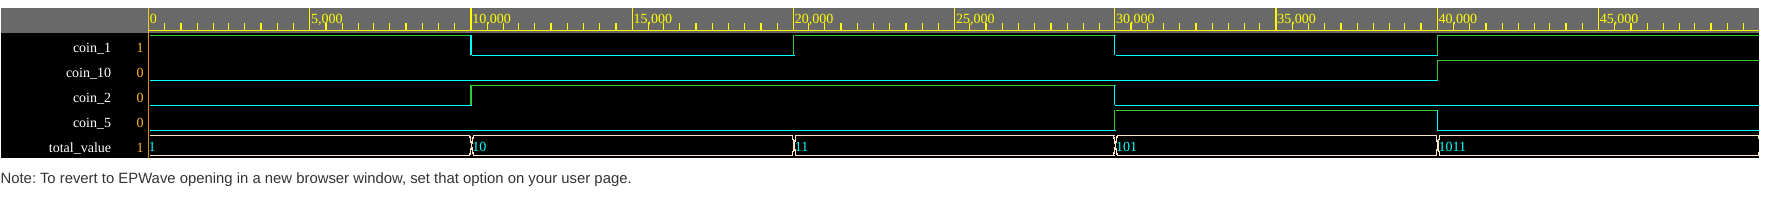
\includegraphics[width=0.75\linewidth]{Imagenes/EPWaves/coin-selector-wave.png}
\end{figure}

\subsubsection{Calculadora de cambio}
La calculadora de cambio es un componente que se encarga de recibir 2 señales de entrada y mandar una señal de salida. Esta señal de salida es la que se encarga de activar el cambio que se debe dar. La calculadora de cambio se encarga de restar el valor de los productos con el valor de las monedas. Simplemente toma el coin\_total y le resta el selected\_product. El código de la calculadora de cambio es el siguiente:

\lstinputlisting[language=VHDL,caption=Calculadora de cambio]{codigos/vhdl/change_calculator.vhd}

Procedimos a probar con los testbench los casos de prueba. Probamos varias combinaciones pero no todas las posibles

\lstinputlisting[language=VHDL,caption=Calculadora de cambio testbench]{codigos/testbench/change_calculator_test.vhd}

Con las EPWaves pudimos comprobar que los casos de prueba funcionaban correctamente.

\begin{figure}[!ht]
  \centering
  \caption{EPWaves de la calculadora de cambio}
  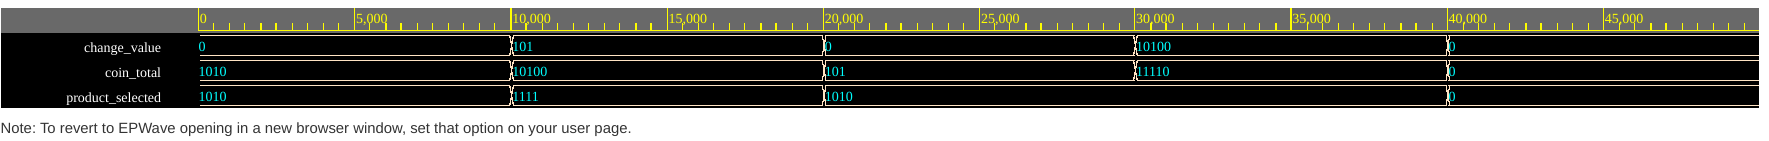
\includegraphics[width=0.75\linewidth]{Imagenes/EPWaves/change-calculator-wave.png}
\end{figure}

\subsubsection{Flip Flop T modificado}
El flip flop T modificado es un componente que se encarga de recibir 2 señales de entrada y mandar una señal de salida. Esta señal de salida es la que se encarga de activar el estado de la máquina expendedora. El flip flop T modificado se encarga de permitir que se pueda comprar algo confirmando la compra. El código del flip flop T modificado es el siguiente:

\lstinputlisting[language=VHDL,caption=Flip flop T modificado]{codigos/vhdl/flipflop.vhd}

Procedimos a probar con los testbench los casos de prueba. Estos casos probamos todo lo que pudimos simulando los cambios de reloj.

\lstinputlisting[language=VHDL,caption=Flip flop T modificado testbench]{codigos/testbench/flipflop_test.vhd}

Con las EPWaves pudimos comprobar que los casos de prueba funcionaban correctamente.

\begin{figure}[!ht]
  \centering
  \caption{EPWaves del flip flop T modificado}
  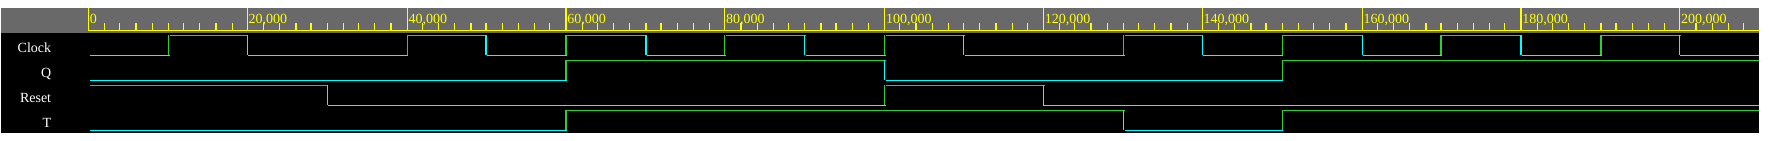
\includegraphics[width=0.75\linewidth]{Imagenes/EPWaves/flipflop-wave.png}
\end{figure}

\subsubsection{Display de 7 segmentos}
El display de 7 segmentos es un componente que se encarga de recibir 2 señales de entrada de tipo número y mandar una señal de salida. Esta señal de salida es la que se encarga de activar el display que se debe mostrar, junto otra que se encarga de decir qué se va a mostrar a detalle. El display de 7 segmentos se encarga de mostrar el valor de los productos y el cambio. Cuando se obtiene el cambio de una compra confirmada se muestra el producto y el cambio si es que se puede comprar el producto. El código del display de 7 segmentos es el siguiente:

\lstinputlisting[language=VHDL,caption=Display de 7 segmentos]{codigos/vhdl/seven_seg_display.vhd}

Procedimos a probar con los testbench los casos de prueba. Estos casos probamos todo lo que pudimos simulando los cambios de reloj.

\lstinputlisting[language=VHDL,caption=Display de 7 segmentos testbench]{codigos/testbench/seven_seg_display_test.vhd}

Con las EPWaves pudimos comprobar que los casos de prueba funcionaban correctamente.

\begin{figure}[!ht]
  \centering
  \caption{EPWaves del display de 7 segmentos}
  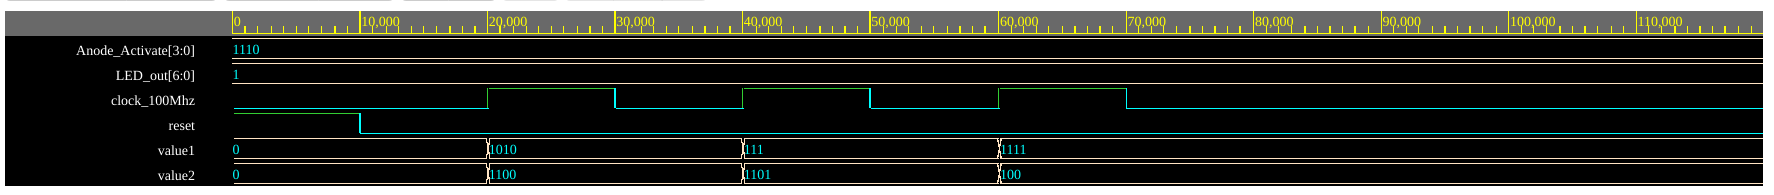
\includegraphics[width=0.75\linewidth]{Imagenes/EPWaves/seven-seg-display-wave.png}
\end{figure}

\subsubsection{Máquina expendedora}
La máquina expendedora es un componente que se encarga de recibir 13 señales de entrada y mandar 2 señales de salida tipo vector. Estas señales de salida son las que se encargan de activar el estado de la máquina expendedora y el producto que se seleccionó. La máquina expendedora se encarga de permitir que se pueda comprar algo confirmando la compra. El código de la máquina expendedora es el siguiente:

\lstinputlisting[language=VHDL,caption=Máquina expendedora]{codigos/vhdl/vending_machine.vhd}

Para este caso no hubo testbench debido a la cantidad de inputs. Se procedió a probar en el Basys 3.

\subsection{Basys 3}
El caso del Basys 3 tenía como propósito hacer las pruebas directas de la máquina. La mayor complejidad recaía en el mapeo. Discutimos la forma de mapear y tuvimos que rediseñar el display; su resultado final es el mostrado en el reporte presente. El mapeo se hizo de la siguiente forma, tal que activaramos el reloj y los displays que eran lo importante en esta parte:

%XDC code
\lstinputlisting[language=VHDL,caption=Basys 3 Master.xdc]{codigos/master.xdc}

Emulamos el circuito en el Basys 3 y probamos los casos de prueba. Escogimos producto 3 y moneda 1 para probar que no se puede comprar con menos dinero que el precio. Pusimos etiquetas de referencia para el usuario. Se buscó poner el botón para confirmar compra como indicaba el reto. El resto son de switches que son en el orden que se pusieron en la etiqueta. R representa el reset y C representa el conseguir el cambio. Las monedas están en la parte derecha y luego siguen los productos posibles.

\begin{figure}[!ht]
  \centering
  \caption{Basys 3 producto 3}
  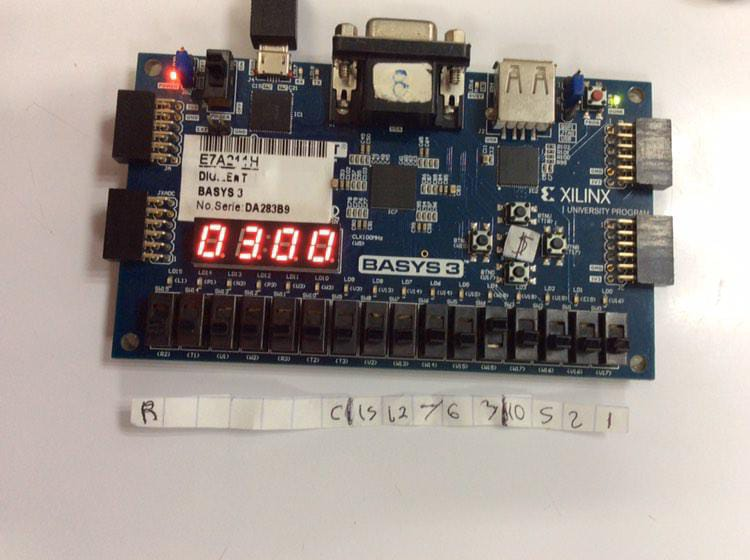
\includegraphics[width=0.75\linewidth]{Imagenes/Basys/product3.png}
\end{figure}

\newpage

\begin{figure}[!ht]
  \centering
  \caption{Basys 3 producto 3 moneda 1}
  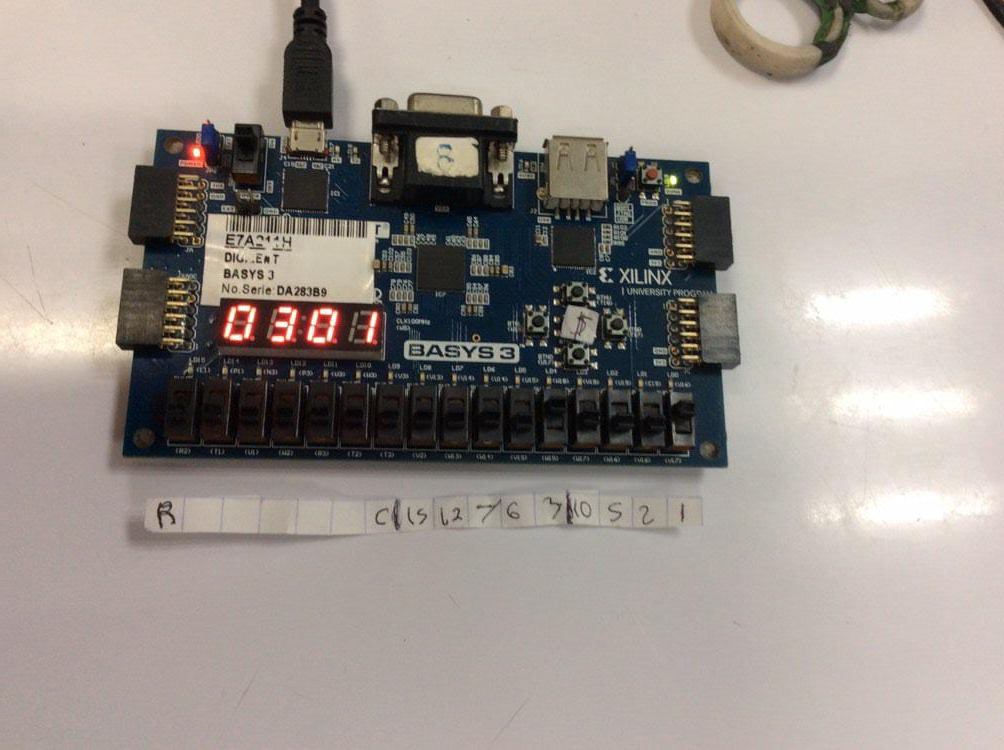
\includegraphics[width=0.75\linewidth]{Imagenes/Basys/product3-coin1.png}
\end{figure}

\begin{figure}[!ht]
  \centering
  \caption{Basys 3 producto 3 moneda 1 confirmar}
  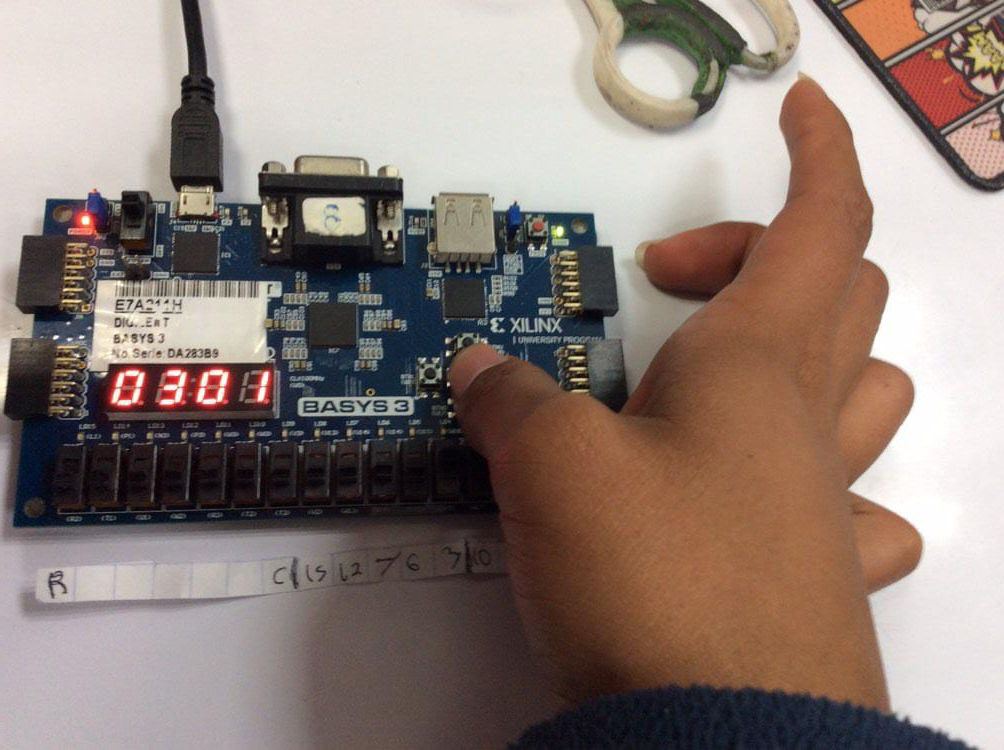
\includegraphics[width=0.75\linewidth]{Imagenes/Basys/product3-coin1-confirm.png}
\end{figure}

\newpage

\begin{figure}[!ht]
  \centering
  \caption{Basys 3 producto 3 moneda 1 confirmado}
  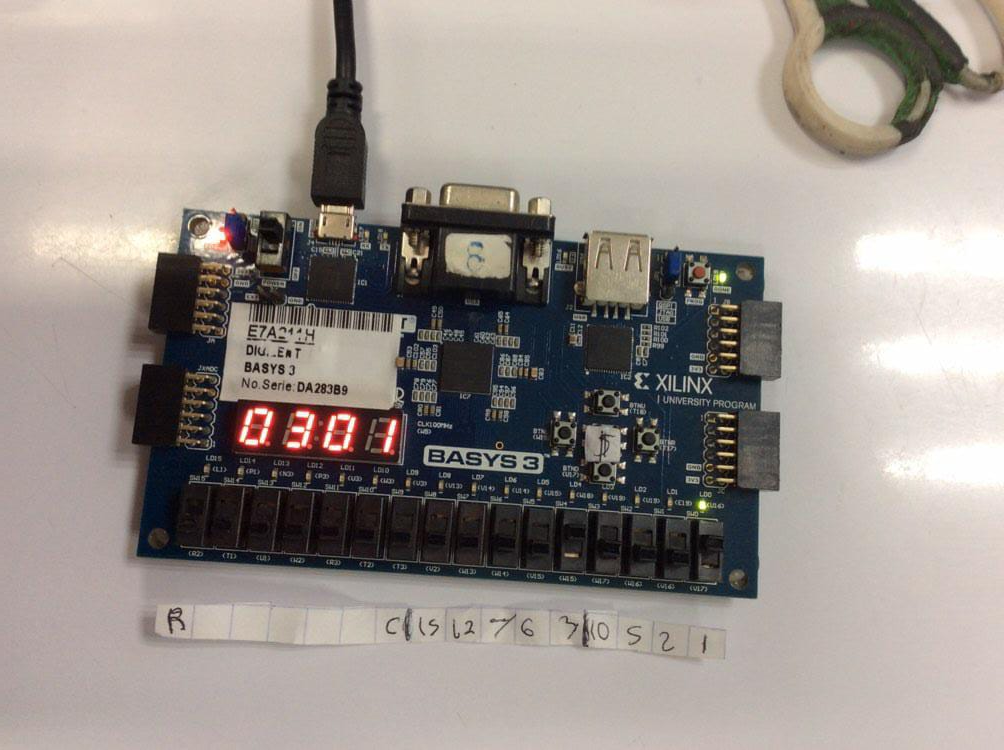
\includegraphics[width=0.75\linewidth]{Imagenes/Basys/product3-coin1-confirmed.png}
\end{figure}

\begin{figure}[!ht]
  \centering
  \caption{Basys 3 producto 3 moneda 1 confirmado sin cambio}
  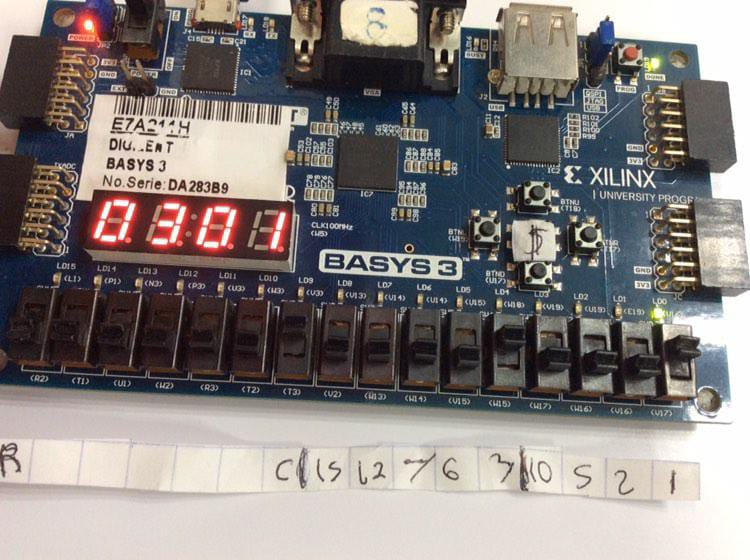
\includegraphics[width=0.75\linewidth]{Imagenes/Basys/product3-coin1-nochange.png}
\end{figure}

Luego confirmamos que se podía comprar con el precio exacto de producto 6 con moneda 5 y moneda 1.

\newpage

\begin{figure}[!ht]
  \centering
  \caption{Basys 3 producto 6 moneda 5 y moneda 1}
  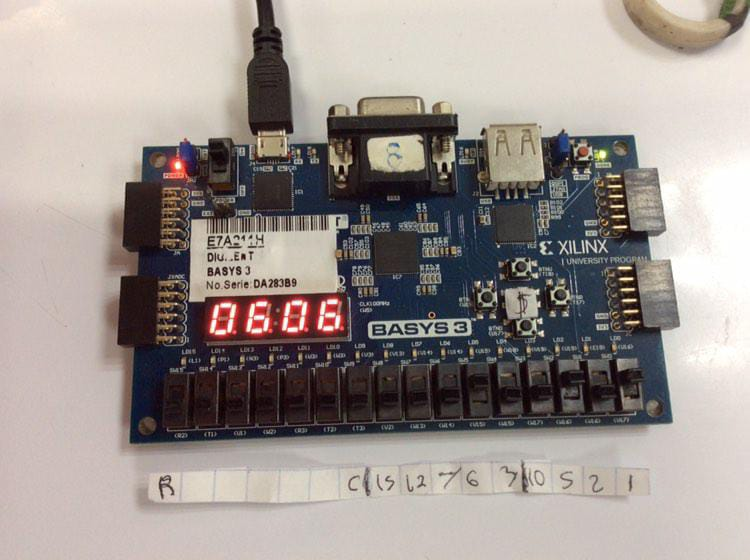
\includegraphics[width=0.75\linewidth]{Imagenes/Basys/product6-coin6.png}
\end{figure}

\begin{figure}[!ht]
  \centering
  \caption{Basys 3 producto 6 moneda 5 y moneda 1 confirmar}
  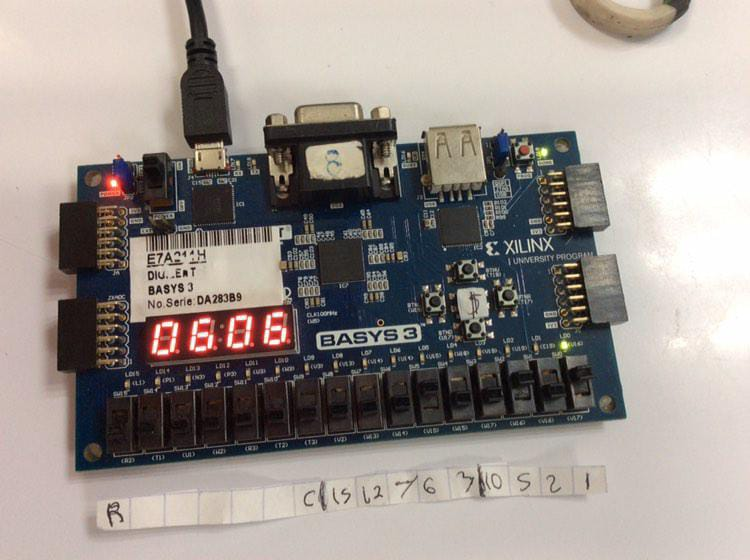
\includegraphics[width=0.75\linewidth]{Imagenes/Basys/product6-coin6-confirmed.png}
\end{figure}

\newpage

\begin{figure}[!ht]
  \centering
  \caption{Basys 3 producto 6 moneda 5 y moneda 1 confirmado}
  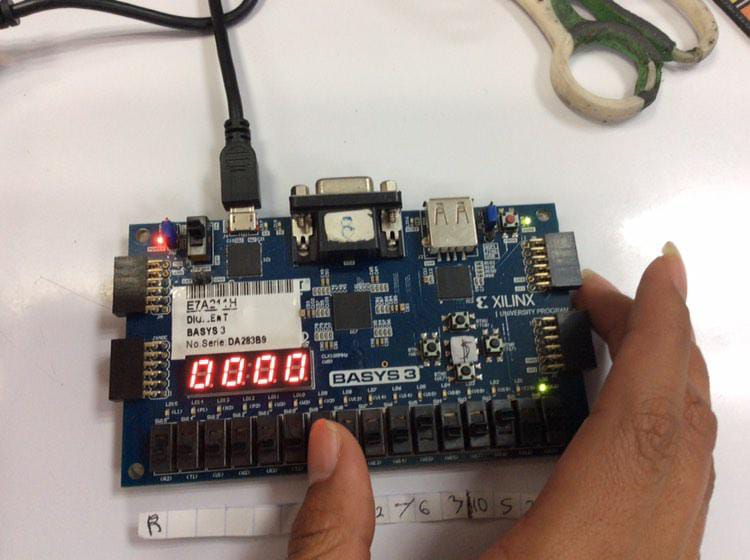
\includegraphics[width=0.75\linewidth]{Imagenes/Basys/product6-coin6-change.png}
\end{figure}

Por último probamos que se podía comprar con más dinero que el precio de producto 7 con moneda 10.

\begin{figure}[!ht]
  \centering
  \caption{Basys 3 producto 7 moneda 10}
  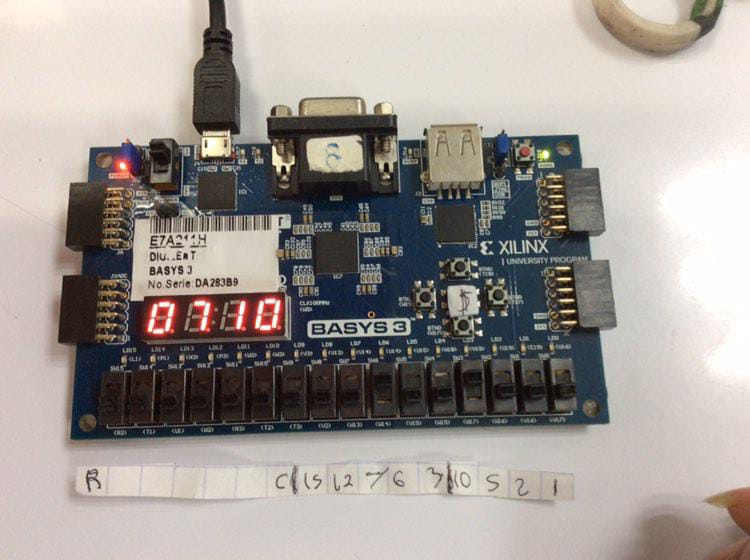
\includegraphics[width=0.75\linewidth]{Imagenes/Basys/product7-coin10.png}
\end{figure}

\newpage

\begin{figure}[!ht]
  \centering
  \caption{Basys 3 producto 7 moneda 10 confirmar}
  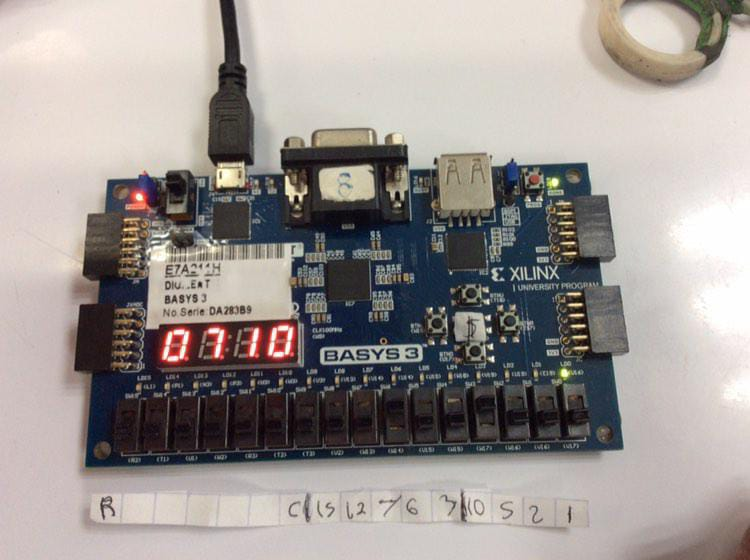
\includegraphics[width=0.75\linewidth]{Imagenes/Basys/product7-coin10-confirmed.png}
\end{figure}

\newpage

\begin{figure}[!ht]
  \centering
  \caption{Basys 3 producto 7 moneda 10 confirmado}
  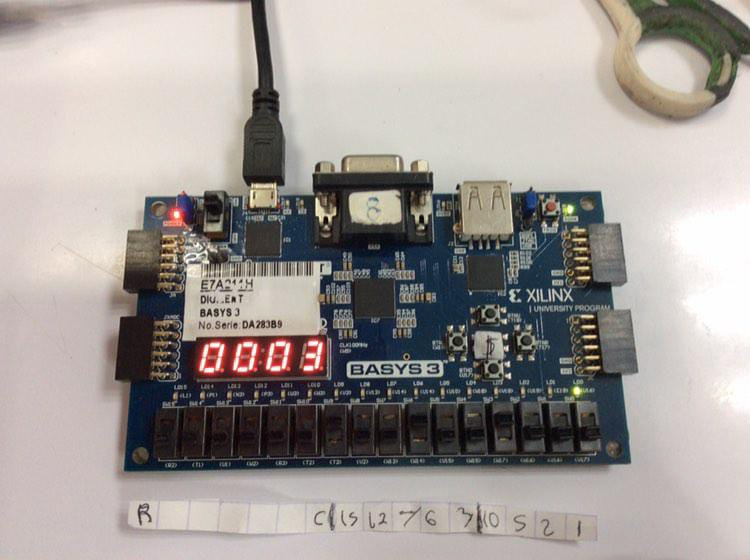
\includegraphics[width=0.75\linewidth]{Imagenes/Basys/product7-coin10-change.png}
\end{figure}

\section{Conclusiones}
En términos de funcionamiento, la máquina cumple el objetivo de permitir comprar. Sin embargo, carece de permitir al usuario el comprar con varias monedas no únicas. Esto se pudo haber conseguido utilizando más flip flops y un sumador de tipo full-adder. La complejidad que se evitó pudo haber permitido realizar el trabajo más realista. Por otro lado, se consiguió un buen resultado para los displays que es algo que se puede llegar a complicar. Como detalles menores, el usuario solo sabe que compró el producto con el cambio, pero sería una adición positiva a la experiencia de usuario haciendo un led que se encienda cuando se haya completado la compra con éxito. Por cuestiones de tiempo y sobre todo la investigación que se hubiera afrontado, se decidió por un sistema secuencial simple donde pudiéramos centrarnos en el display y el reloj que nos hicieron rediseñar el circuito dos veces.

\newpage %Termina la pagina y empieza una nueva
\appendix % A partir de este comando, todas las


%%%%%%% Bibliografía %%%%%%%%
\clearpage %Asegura que la bibliografía inicie en una nueva página
\bibliographystyle{bst/IEEEtran} %Estilo de bibliografía
\bibliography{bib/bibliografia} %Fuentes bibliográficas
\addcontentsline{toc}{section}{Referencias}  %Agrega la bilbiogrfía al indice
%%%%%%% Bibliografía %%%%%%%%      
\end{document} %Termina el documento